\chapter{Results}\label{cha:results}
\section{Simulation experiments}
The proposed framework was evaluated by performing a number of simulations in the ArduPlane \ac{sitl} environment, in different wind conditions. 
Some resulting landings can be seen in Figure \ref{fig:sim_sol_0}-\ref{fig:sim_sol_270}. The parameters used during these simulations are summarized in Table \ref{tab:sim_params}.

\begin{table}[H]
    \begin{center}
        \begin{tabular}{|c|c|c|}
            \hline
            \textbf{Parameter} & \textbf{Value} & \textbf{Description}\\
            \hline
            $x_0$ & $(0,0,0\degree)$ & Initial state \\
            \hline
            $\airspd$ & 14 m/s & Airspeed \\
            \hline
            $\windspd$ & 5 m/s & Wind speed \\
            \hline
            $h_0$ & 40 m & Initial altitude \\
            \hline
            $h_{\text{safe}}$ & 10 m & Landing area safety altitude \\
            \hline
            $\flarealt$ & 3 m & Flare altitude \\
            \hline
            $\flaresink$ & 0.5 m/s & Flare sink-rate\\
            \hline
            $\dot{h}_{\text{max}}$ & 3 m/s & Maximum sink-rate \\
            \hline
            $\dot{\psi}_{\text{max}}$ & $17\degree$/s & Maximum rate of turn\\
            \hline
            $\psi_{L,d}$ & $10\degree$ & Approach direction discretization \\
            \hline
        \end{tabular}        
    \end{center}
    \caption{Simulation parameters}
    \label{tab:sim_params}
\end{table}

\begin{figure}[H]
    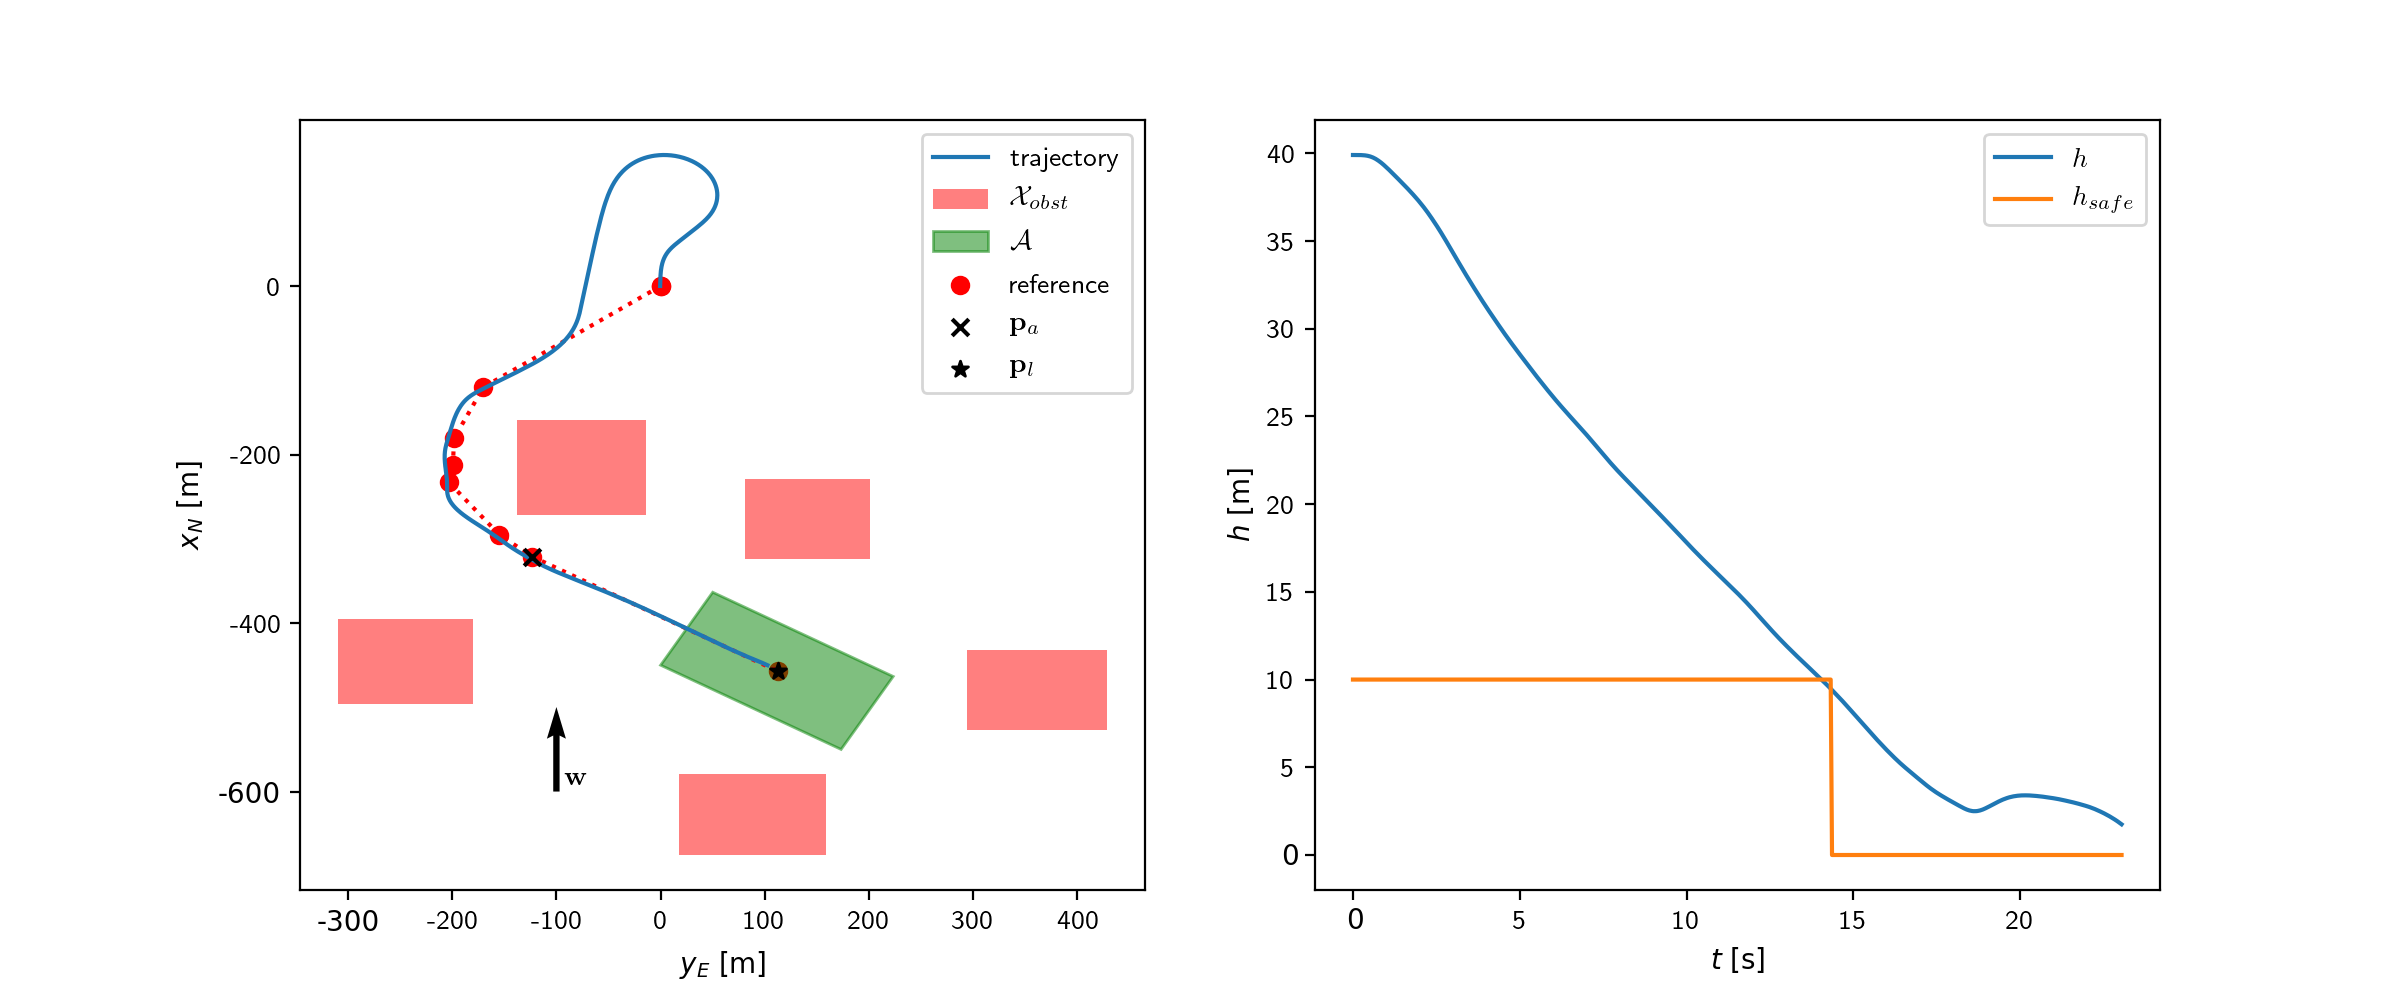
\includegraphics[width=\linewidth]{sol_0}
    \caption{Landing sequence and altitude profile for $\winddir=0\degree$}
    \label{fig:sim_sol_0}
\end{figure}

\begin{figure}[H]
    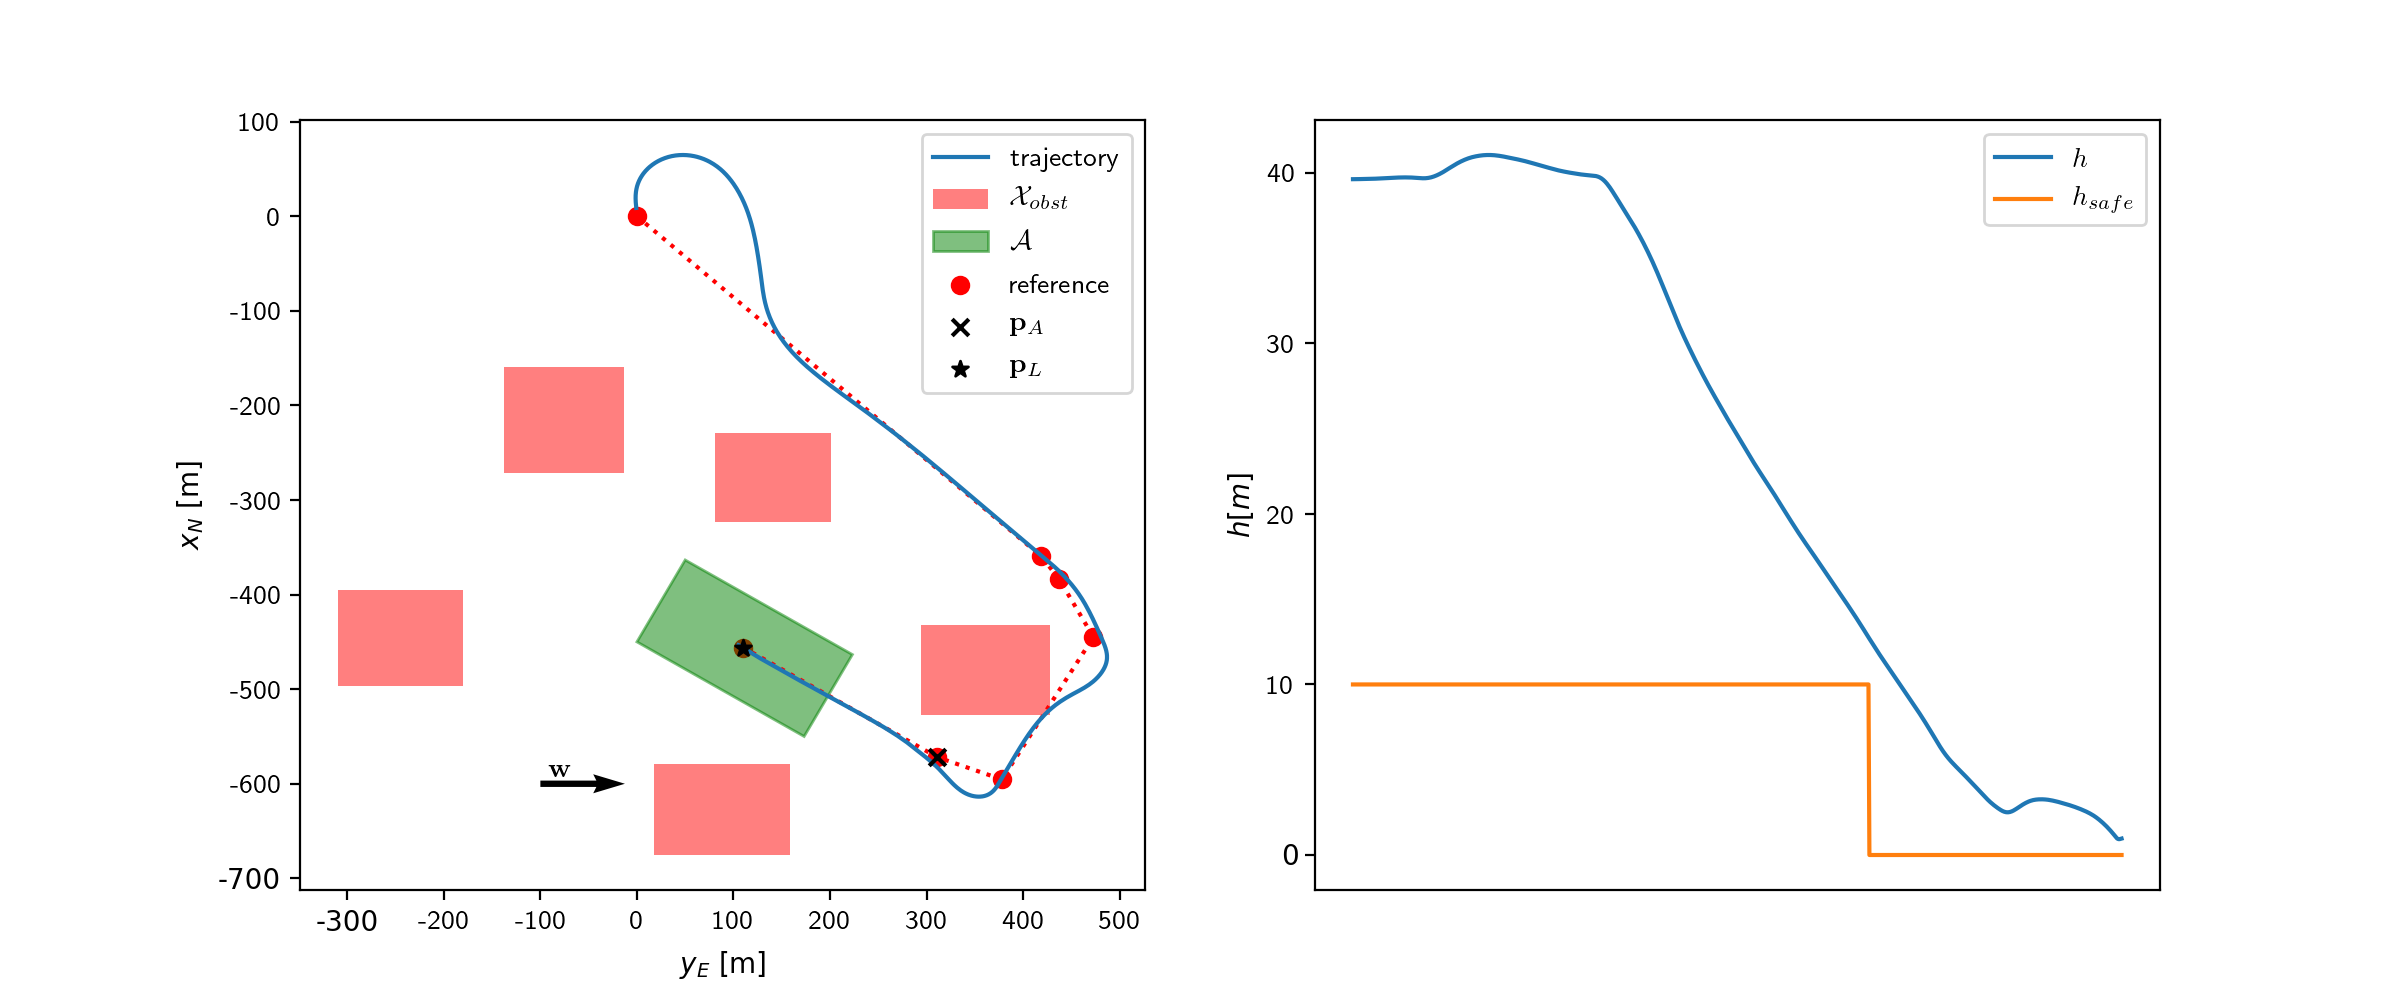
\includegraphics[width=\linewidth]{sol_90}
    \caption{Landing sequence and altitude profile for $\winddir=90\degree$}
\end{figure}

\begin{figure}[H]
    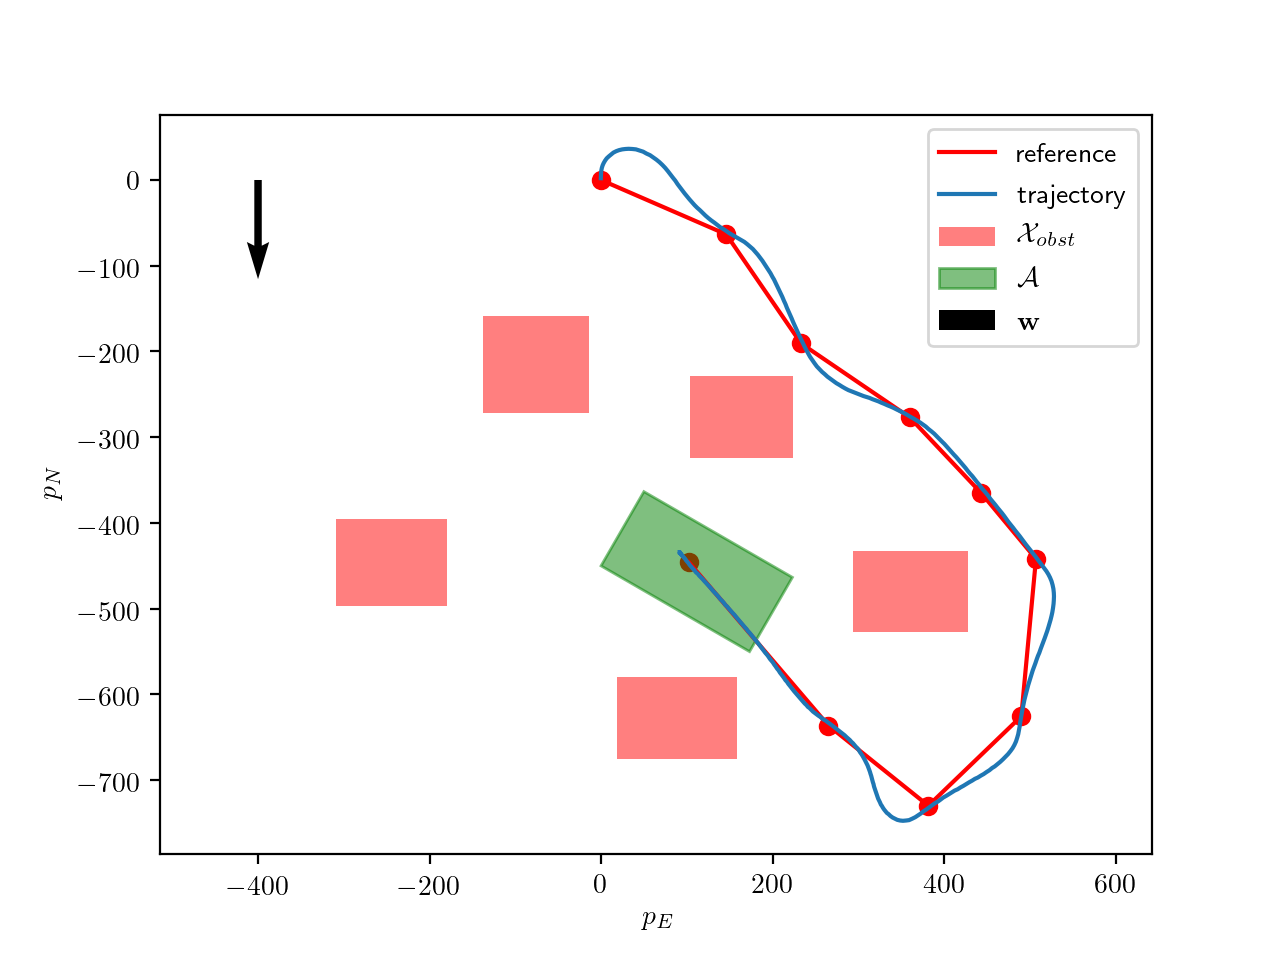
\includegraphics[width=\linewidth]{sol_180}
    \caption{Landing sequence and altitude profile for $\winddir=180\degree$}
\end{figure}

\begin{figure}[H]
    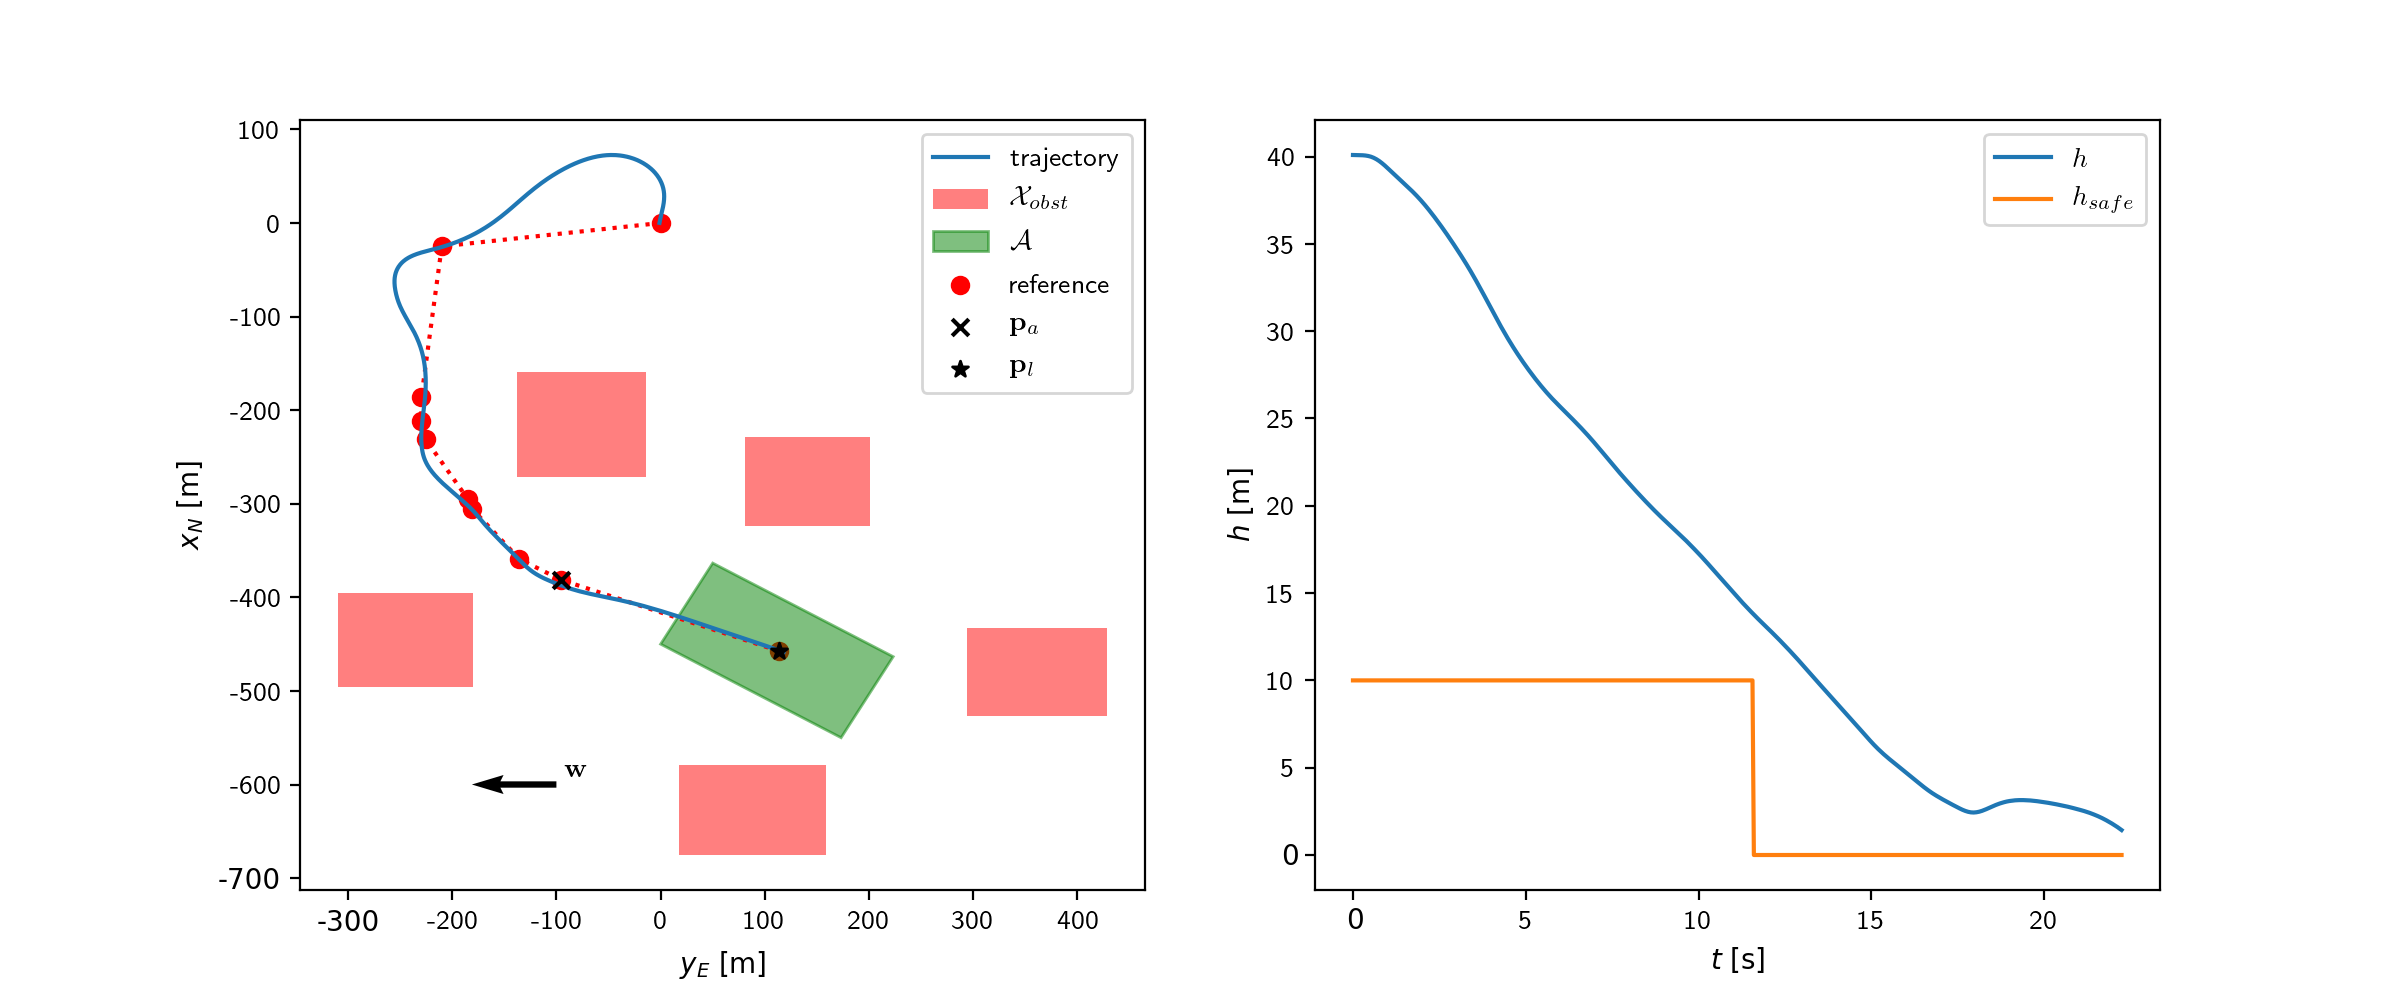
\includegraphics[width=\linewidth]{sol_270}
    \caption{Landing sequence and altitude profile for $\winddir=270\degree$}
    \label{fig:sim_sol_270}
\end{figure}


Some relevant properties of the different solutions are summarized in Table \ref{tab:opt_land_param}. $\psi_L^*$ and $R_a^*-R_l^*$ is the optimal approach direction and total landing distance for each given $\winddir$. $h_A^*$ and $|R_l^*-R_c|$ is the calculated entry altitude and distance from the landing point to the center of $\landing$. 
$h_A$ is the actual entry altitude and $|R_l-R_l^*|$ the distance from the calculated landing point to the actual touchdown point of the \ac{uav}, both obtained from the simulation. Finally, $T$ is the
execution time of the entire landing sequence calculation.

\begin{table}[H]
    \begin{center}
        \begin{tabular}{|c|c|c|c|c|c|c|c|c|}
            \hline
            $\mathbf{\winddir}$ & $\mathbf{\psi_L^*}$ & $\mathbf{R_a^*-R_l^*}$ & $\mathbf{h_A^*}$ & $\mathbf{h_A}$ & $\mathbf{|R_l^*-R_c|}$ & $\mathbf{|R_l-R_l^*|}$ & $\mathbf{T}$\\
            \hline
            $0\degree$ & $120\degree$ & 272 m & 17.09 m & 9.4 m & 0.95 m & 4.84 m & 0.04 s \\
            \hline
            $90\degree$ & $300\degree$ & 232 m & 19.45 m & 12.68 m & 1.49 m & 5.87 m & 0.32 s \\
            \hline
            $180\degree$ & $320\degree$ & 244 m & 19.64 m & 11.5 m & 1.44 m & 1.48 m & 0.97 s \\
            \hline
            $270\degree$ & $110\degree$ & 222 m & 20.4 m & 13.76 m & 1.71 m & 5.92 m & 0.08 s \\
            \hline
        \end{tabular}
    \end{center}
    \caption{Landing sequence solution properties}
    \label{tab:opt_land_param}
\end{table}

\section{Real flight experiments}